\chapter{Experiment Characterisation}

    Before we can dive into running novel experiments involving the motion and spin
    of the atoms, we need to characterise our apparatus. This allows us to both
    benchmark our system against state of the art results, and to reveal any
    current limitations of the apparatus which we may need to address.

\section{Quadrupole Transitions}
\label{sec:Transitions}
% Main points:
    % All visible motional modes on large detuning scan at $5$~G. 
    % Can compare when have all quadrupole transitions available or when we selectively omit transitions via polarisation.
% Pre reqs:
    % 5 G field

\section{Spin}
\label{sec:Spin}

\subsection{Rabi and Ramsey Scans}
% Main points:
    % The ion is a sensor!
    % Method for Rabi and Ramsey scans
    % Mention changing polarisation to select certain transitions
    % Long Rabi flop
    % Likely reason for flop damping
    % Measuring detuning using Ramsey scan
% Pre reqs:
    % 729 system
    % Available Quadrupole transitions

    \begin{figure}
        \begin{center}
        \noindent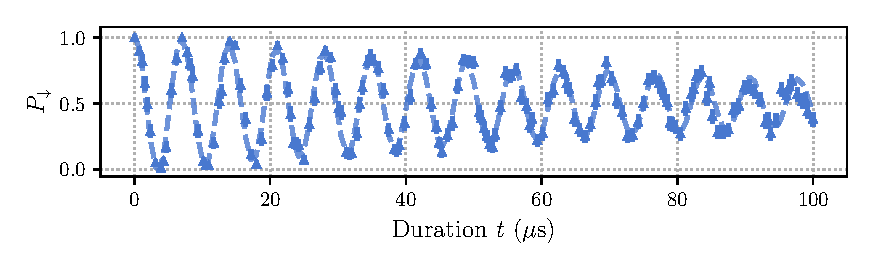
\includegraphics[width=\linewidth]{
            figures/pdf_figure/long_flop.pdf
            }
        \end{center}
        \caption{Long duration Rabi Flop with fitted decaying flop.
            }
        \label{fig:Long Flop}
    \end{figure}

    Here we briefly describe the method in which we extract Rabi frequencies and single qubit gate durations.
    Long Rabi flop (100 us), fit out carrier frequency of 2*pi*0.0716(1) MHz and
    Decay rate of $0.0107(7)$ 1 / us. See long flop. This is 1 mW of power on m1\_m3
    transition before we changed polarization. Fit with decaying cos function 
    \begin{equation}
        \frac{1 + e^{-\lambda t} \cos(2 \Omega t)}{2},
    \end{equation}
    % 1 mW 729~nm laser -> Fit out pi/2, pi, 2pi pulses. We are using square pulses.


\subsection{Spin Coherence Times}
\label{sec:Coherence}
% Main points:
    % Quote coherence times comparing:
        % Mumetal box panels
        % Transitions with diff mag sensitivity
        % FNC/ no-FNC
% Pre reqs:
    % MuMetal box
    % Available transitions
    % 729 laser system

    Individual gate fidelities are ultimately limited by loss of coherences of
    the two qubit states due to either dephasing or by the natural lifetime of the upper level. By our choice of ion and qubit levels, defined between
    the ground $4S_{1/2}$ state and the metastable $3D_{5/2}$ state, we can
    expect a lifetime limited coherence time of $\tau = 1.1$~s~\cite{}. 
    %Barton, P. A. et al. Measurement of the lifetime of the 3d 2D5/2 state in
    %40Ca+.Physical Review A 62, 032503 (2000).
    In practise, mainly due to imperfect tracking of laser frequency and
    magnetic field drifts (as mentioned above), we see coherence times dominated
    by dephasing. To discern between these two noise sources, we may exploit the
    fact that we have multiple Zeeman levels within our $3D_{5/2}$ state with
    varying magnetic field sensitivities. We also have the ability to define our
    qubit on the Zeeman split ground state, which decouples dephasing due to the
    laser from measured coherence times. We perform Ramsey scans with varying
    mid-sequence delay durations to extract the coherence times, an example of
    which can be seen in figure~\ref{fig:coherence_times}. In characterising the
    spin coherence times, we hope to explore both the efficacy of the magnetic
    shielding surrounding the ion trap, as well as the stability of the 729~nm
    laser. \\
    Figure~\ref{fig:coherence_times} shows how the magnetic shielding effect
    coherence times of three transitions, XX, YY and ZZ, with magnetic field
    sensitivities of XX, YY and ZZ respectively.  From this we find that without
    the shielding, we are strongly limited by external magnetic field noise, and
    with full sheilding we suppress this noise to where we are dominated by
    laser phase noise. To find the factor by which the magnetic field noise is
    attenuated, we can compare the coherence times of the laser phase
    insensitive transition with and without the box. We find an attenuation
    factor of XX, which is XXconsisitent with the expected attenuation factor of
    the mu-metal shielding.\\
    With the shiedling in place, we compare the coherence times of the
    $4S_{1/2}, m_j = -1/2 \leftrightarrow 3D_{5/2}, m_j = -5/2$ with fibre noise cancellation (see
    section~\ref{sec:Narrow Line Width 729 Laser}) and without, figure~\ref{fig:coherence_times}. We find that the
    coherence time is improved by a factor of XX, with FNC enabled. Our current
    spin coherence time of XX~ms is limited by the laser phase noise, and we
    expect to be able to push this to [ref R. Oswald] by improving the laser PDH
    stability. However, for the immediate planned experiments (see
    section~\ref{Outlook}), these improvements will be a low priority due to
    other likely dominating error sources in the motion of our ions.\\

\subsection{State Preparation and Measurement}
% Main points:
    % Method of preparation via optical pumping
    % Readout characterisation with NA 0.6 lens
    % Compare readout histograms of fast 30 us readout to Doppler cold 100 us readout
    % Quote state prep error (back this from RBM + measurement histograms)
% Pre reqs:
    % Laser systems powers
    % 729 system
    % Available transitions
    % pi-pulses

    To utilise two levels of the ion as a qubit, we need to be able to
    selectively prepare the ion into one of the Zeeman levels of the ground
    state. As mentioned in section~\ref{sec:Magnetic Field}, we are operating at
    a low magnetic field of 5~G, leading to a splitting between the Zeeman
    levels of less than 21~MHz, the natural linewidth of the 397~nm transition.
    This means we cannot optically pump using 397~nm frequency selectivity.
    Further, due to the constraint of beam geometry from the in vacuum optics,
    we can not use polarisation selectivity of the 397~nm transition. Instead,
    we use the narrow line width 729~nm laser on resonance with the $4S_{1/2},
    m_j = +1/2 \leftrightarrow 3D_{5/2}, m_j = -3/2$ transition, and the 854~nm
    deshelving laser on resonance, to optically pump into the $m_j = -1/2$
    Zeeman level we define as our qubit ground state. \\
    To measure the qubit state of the ion, we apply the 397~nm and 866~nm lasers
    and count 397~nm photons scattered. From the level diagram shown in
    figure~\ref{fig:level_diagram}, we can see that upon turning on the 397~nm
    laser, if we are in $|0\rangle$, photons will be scattered, and if we are in
    $|1\rangle$, then no photons will be scattered. To optimise the fidelity of
    measurement we ensure that the signal is discernible with low error from any
    background counts on the camera. In general, improving the number of signal
    counts can be achieved by tuning the 397~nm laser near to the transition
    resonance, by increasing the readout duration, or by increasing the
    percentage of scattered photons captured by the imaging system. Practically
    we desire that the readout step does not heat the motion of the ion and so
    we red detune the 397~nm laser to a similar setting as for Doppler cooling
    (see section~\ref{sec:Cooling}). The parameters we use for readout are
    summarised in table~\ref{tab:readout_parameters}, and a typical histogram of
    readout counts for one and two ions can be seen in
    figure~\ref{fig:readout_histogram}. We find that the readout fidelity is
    XXX.\\
    To measure the effect of state preparation and measurement error on longer
    experimental sequences, we will discuss randomised benchmarking in the following
    section~\ref{sec:Randomised Benchmarking}. Due to the relevance here, we
    quote the measured state-preparation and measurement error (SPAM) of $\epsilon_{SPAM} = 1.46(6) \times 10^{-3}$.\\
    
\subsection{Randomised Benchmarking}
\label{sec:Randomised Benchmarking}
% Main points:
    % Here is a characterisation of single qubit gates.
    % Explain RBM method
    % Quote values measured
    % What is likely error source
    % Are we limited by this error?
    % What is state of the art (for optical quadrupole transition)
    % What contribution is the spin coherence time?
% Pre reqs:
    % Spin coherence times
    % Possible transitions
    % Calibrating gate times

    \begin{figure}
        \begin{center}
        \noindent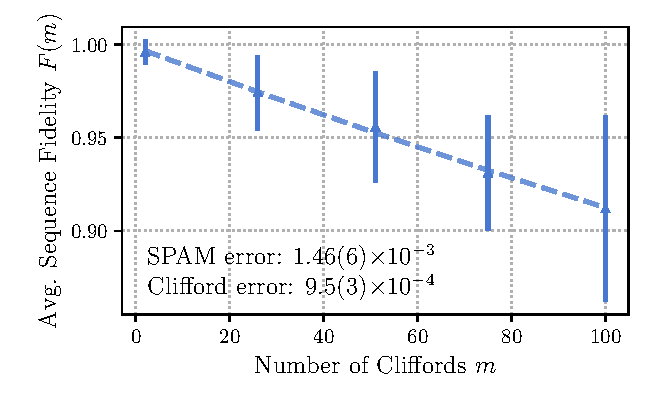
\includegraphics[width=\linewidth]{
            figures/pdf_figure/rbm_fit.pdf
            }
        \end{center}
        \caption{
            RBM fit
            }
        \label{fig:rbm}
    \end{figure}

    High fidelity unitary operations (gates) are essential for both near
    intermediate scale quantum computing and for reducing overheads in required
    physical qubits and operations in fault-tolerant
    schemes~\cite{steane_overhead_2003}. To evaluate the quality of both our
    state-prep and single qubit rotations, we employ randomized benchmarking
    (RBM)~\cite{knill_randomized_2008, magesan_scalable_2011}.  RBM consists of
    applying random combinations of a pre-chosen discrete set of gates to
    estimate an average error per gate.  We chose the single-qubit Clifford
    group as our set of gates to evaluate. The single-qubit Clifford group is
    the set of unitaries which map the Pauli matrices to one another through
    conjugation. This can be thought of as the complete set of rotations of the
    Bloch sphere such that all valid combinations of the axis $(x \rightarrow
    \{\pm x,~\pm y,~\pm z\}),~(y \rightarrow \{\pm x,~\pm y,~\pm z\}),~(z
    \rightarrow \{\pm x,~\pm y,~\pm z\})$ are realized. There are 24 unitaries
    in this set. We followed the RBM protocol described in the
    Thesis~\cite{hughes_benchmarking_2021} to evaluate our single-qubit gates.
    First the qubit is prepared in some known initial state, i.e. prepared in
    some chosen basis. A gate sequence is then applied which consists of
    multiple random Clifford gates followed by a final `inverting' Clifford,
    where the `inverting' Clifford is chosen such that the full sequence
    performs the Identity operation. The state is then measured in the same
    basis to find any deviations from the Identity being performed due to gate
    errors. This is repeated with the same preparation and sequence multiple
    times to calculate the probability that the Identity was performed - thus
    giving the sequence fidelity. These steps are repeated for many different
    random sequences with a range of sequence lengths. The decay model we fit to
    the fidelity versus number of Clifford gates is given by,

    \begin{equation}
        F(m) = \frac{1}{2}\left( 1+(1-2\epsilon_{SPAM})(1-2\epsilon_c)^m\right),
    \end{equation}

    \noindent where $F(m)$ is the fidelity of the sequence of length $m$,
    $\epsilon_{SPAM}$ is the state-preparation and measurement error, and
    $\epsilon_c$ is the average error per Clifford gate.  We use this method to
    bench mark our qubit transition. The Clifford gates are decomposed into
    sequences of $\pi/2$ and $\pi$ pulses about either the $x-$ or $y-$axes. We probe up to $m=100$ Clifford gates, and fit the decay of the fidelity to the above model.
    We measure the error per Clifford to be $\epsilon_c = 9.5(3) \times 10^{-4}$,
    while the SPAM error is $\epsilon_{SPAM} = 1.46(6) \times 10^{-3}$. The decay plot for
    this RBM sequence can be seen in figure~\ref{fig:RBM_decay}. The error bars
    are given by the standard deviation of the survival populations. There are on average 3.50 $\pi/2$ pulses per Clifford, with a typical $\pi/2$ duration of $1.3~\mu$s.\\


\section{Motion}
\label{sec:Motion}
% Main points:
    % Quote characterisation method and values for various motional measurements.
    % Highlight where we are not yet at the capability we need.
    % State what improvements we plan to add.
% Pre reqs:
    % Motivation for control of motion of ion
    % Trap RF DC
    % Laser systems

\subsection{Cooling}
\label{sec:Cooling}
% Main points:
    % Introduce why we want to cool
    % Doppler cooling
    % Sideband cooling
% Pre reqs:
    % Motional mode and beam geometry
    % Laser systems 
    % Trapping

    For any interaction involving the motion of the ion, we require both the
    ability to prepare the motional state with high fidelity, and to
    subsequently measure this motional state to verify correct preparation. For
    entangling gates, and the creation of squeezed states which we are
    considering in this chapter, we assume that we begin in the motional ground
    state, or in other words, Fock state zero.  Our initially trapped ions will
    be in some high temperature thermal state, (*given by the oven temperature
    and the PI laser momenta kicks*). We first doppler cool our ions, and then
    subsequently sideband cool them. We give a brief description of these two
    cooling processes here.\\

\subsubsection{Doppler Cooling}
% Main points:
    % Quote final temperature reached (theory?)
    % Describe cooling parameters
% Pre reqs:
    % Motional mode and beam geometry
    % Laser systems 

    Doppler cooling exploits the fact that incident light onto a moving ion will
    appear frequency shifted in the rest frame of the ion. For Doppler cooling
    of $^{40}$Ca$^+$, we apply both the 397~nm and 866~nm lasers. We initially red
    detune the 397~nm laser by around 100~MHz. This results in the preferential
    absorption of a quanta of 397~nm light by ions with a velocity vector
    antiparallel photon k-vector. After this absorption, the ion will be in the
    excited $4P_{3/2}$ state and spontaneously decay to either the $4S_{1/2}$,
    or the $3D_{3/2}$ emitting a photon of either 397~nm or of 866~nm
    respectively into a random direction. These two decay paths have a branching
    ratio of XX.  As we desire many photon kicks to cool our ions, we repump the
    electron out of this metastable $3D_{3/2}$ level by applying an on resonant
    866~nm beam.  The absorption and sequential emission of this 397~nm photon
    will lead to a net reduction in the motional energy of the ion if the photon
    is emitted at a higher energy than when absorbed. The equilibrium
    temperature is given by the condition where the doppler cooling rate is
    equal to photon recoil heating of the ion. Assuming a Lorentzian absorption
    profile, the minimum temperature is given by,
    \begin{equation}
    T_{Doppler} \approx \frac{\hbar\gamma}{2k_B},
    \end{equation}
    where $\hbar$ is the reduced Planck constant, $\gamma$ is the natural
    linewidth of the transition, and $k_B$ is Boltzmann's constant.\\ For
    $^{40}$Ca$^+$, the natural linewidth of the 397~nm transition is $\frac{\gamma}{2\pi} =
    21$~MHz, leading to a Doppler temperature of approximately 0.5~mK. Given a radial mode frequency of $\frac{\omega}{2\pi} = 4$~MHz, and the mean occupation number of the oscillator being given by,
    %[ref NIST https://www.physics.nist.gov/PhysRefData/Handbook/Tables/calciumtable4.htm] 
    \begin{equation}
        \bar{n} = \frac{1}{e^{\hbar\omega/k_B T}-1},
    \end{equation}
    we find the final thermal distribution to have an expected Fock state of $\bar{n} = 2.3$.
    Using parameters summarised in table~\ref{tab:cooling_parameters}, we find practically the final temperature after Doppler cooling to be around XXX~mK.\\

\subsubsection{Sideband Cooling}
% Main points:
    % Quote final temperature reached
    % Describe SBC pulse sequence
    % We use a closed transition
% Pre reqs:
    % Motional mode spectra
    % Laser systems 
    % Rabi flopping

    \begin{figure}
        \begin{center}
        \noindent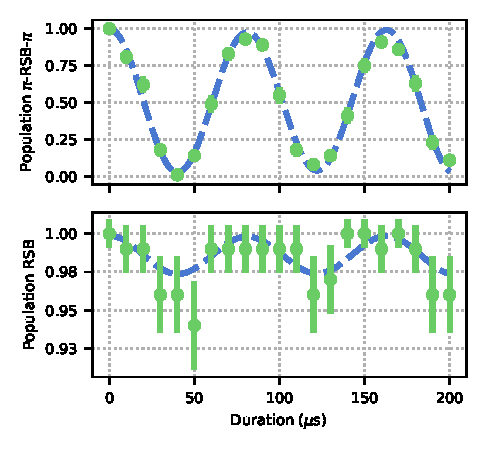
\includegraphics[width=\linewidth]{
            figures/pdf_figure/sideband_thermometry.pdf
            }
        \end{center}
        \caption{
            Thermometry after sideband cooling.
            }
        \label{fig:SBC}
    \end{figure}

    \begin{figure}
        \begin{center}
        \noindent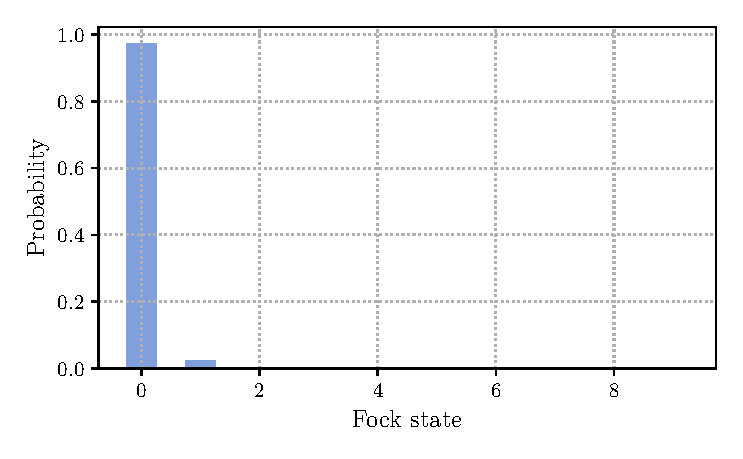
\includegraphics[width=\linewidth]{
            figures/pdf_figure/fock_state_distribution.pdf
            }
        \end{center}
        \caption{
            Fock state distribution
            }
        \label{fig:fock state}
    \end{figure}


    To further cool the ions toward their motional ground state, we use resolved
    sideband cooling. The motion of the ion, described by a harmonic oscillator,
    modulates the transition frequencies of the ion, leading to sidebands at
    multiples of the motional frequency. For the $4S_{1/2} \leftrightarrow
    3D_{5/2}$ transition, at appropriate laser intensity and motional mode
    frequencies, these sidebands can be resolved spectroscopically. The pulsed
    sideband technique we employ consists of red sideband pulses, followed by
    deshelving, and repumping pulses on the 854~nm and 866~nm transitions
    respectively. An example pulse sequence can be seen in
    figure~\ref{fig:sideband_cooling_sequence}, and experimental parameters we use are summarised in table~\ref{tab:cooling_parameters}.\\
    To verify the efficacy of our sideband cooling, we perform thermometry
    experiments by driving on resonance red sideband (RSB) and pi-RSB-pi pulse
    sequences. We record the time dynamics of population flopping as we vary RSB
    pulse length. In the case of Fock state zero, we expect to see a strong
    signal on the RSB, and no signal on the pi-RSB-pi pulses. We fit a thermal
    Fock state distribution (with truncation at Fock state = 100) to these
    signals to extract the mean occupation number, and $\eta\Omega$, the carrier
    Rabi frequency multiplied by the Lamb-Dicke parameter. A typical thermometry
    scan after Doppler and sideband cooling can be seen in
    figure~\ref{fig:sideband_cooling_results}. We find that the mean occupation
    number after sideband cooling is $\bar{n} = 0.03()$, and $\eta\Omega =
    XX$~MHz.\\
    Optimisation of the cooling parameters can be roughly performed by fitting
    temperature while scanning RSB pi-pulse durations, total number of pulses,
    repumping and deshelving times. One can optimise for minimum temperature,
    however it is also important to optimise for total cooling duration. For
    single ion, single mode experiments, this duration is often a non-issue,
    however for multi-ion crystals, any interaction involving the motion, may
    require the sequential sideband cooling of multiple motional modes. This can
    not be easily parallalised due to the requirement that the RSB pi-pulse is
    performed near resonance to one of the motional sidebands. This sequential
    cooling strategy can be either limiting when heating and cooling rates are
    comparable, or in the best case, painful due to long data collection times.\\
    To mitigate this issue, other sub-Doppler cooling techniques with larger
    accepted frequency bandwidths may be employed. Examples are dark-resonance
    cooling[], and electromagnetically induced transparency (EIT) cooling[], and
    Sisyphus cooling[]. These techniques are not yet implemented in our system,
    but will be likely additions once we move to larger ion crystals.\\

\subsection{Heating Rates}
\label{sec:Heating}
% Main points:
    % Quote motional heating rates for mode we use (have access to).
    % Describe heating model?
% Pre reqs:
    % Thermometry
    % Motional modes
    % Trap

    \begin{figure}
        \begin{center}
        \noindent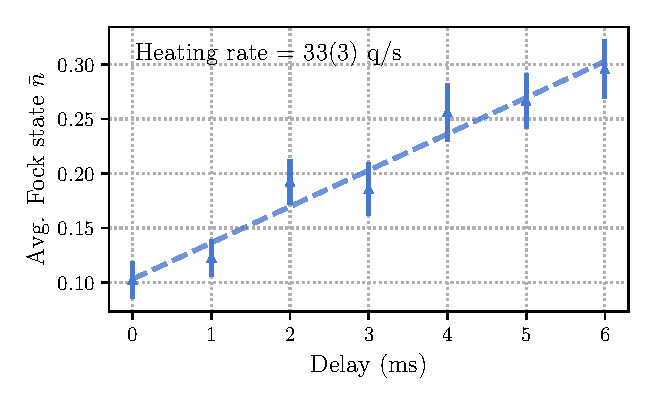
\includegraphics[width=\linewidth]{
            figures/pdf_figure/heating_rate.pdf
            }
        \end{center}
        \caption{
            Heating rates of upper radial mode.
            }
        \label{fig:heating rates}
    \end{figure}

    As mentioned, the cooling of our ions is only relevant if we have acceptable
    heating rates. Heating of the motion is predominantly caused by the ion trap
    itself. This can be due to imperfections in the surface of exposed
    dielectric and metals causing stray fields, or can be due to noise on the DC
    and RF drive voltages[]. Noise due to the surface of the trap can be
    mitigated by increasing ion-electrode distances, or by using traps with
    smaller surface area direclty exposed to the ion. In our case, as mentioned
    in sections~\ref{sec:The Ion Trap}, the NPL trap has an electrode ion
    distance somewhat larger than most surface traps, but less than that of a
    macroscope blade or rod style trap. To verify the heating rate of our
    system, we performed a series of thermometry scans whilst varying some delay
    time between cooling and thermometry pulses. A typical plot can be seen in
    figure~\ref{fig:heating_rate}. We find that the heating rate of our system
    is approximately $33(3)$~quanta per second on the upper radial 4~MHz mode on
    one ion.\\
    It is expected that the heating rate will be larger for lower frequency
    motional modes if we assume uniform electric field noise. We also verify
    this by looking at heating rate on the radial mode while varying the axial
    mode frequency. This is a useful diagnostic to check for unexpected heating
    at certain frequencies, perhaps due to RF noise in the lab. We find....\\

\subsection{Motional Mode Stability}
% Main points:
    % Quote motional mode drift 
    % Explain why it is currently drifty
    % Outline how this will be improved with the squareatron
% Pre reqs:
    % Trap

    \begin{figure}
        \begin{center}
        \noindent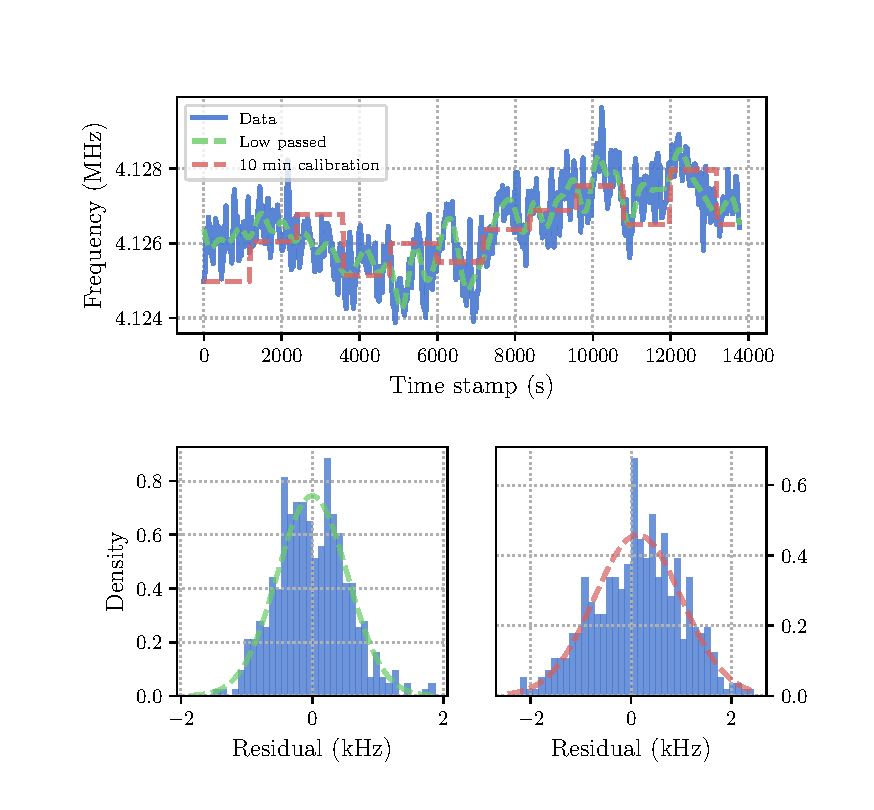
\includegraphics[width=\linewidth]{
            figures/pdf_figure/mode_drift.pdf
            }
        \end{center}
        \caption{
            Motional mode frequency drift.
            }
        \label{fig:mode drift}
    \end{figure}

\subsection{Motional Coherence Times}
% Main points:
    % Quote measured result for motional coherence time
    % Give estimate for what times we need for future experiments
    % Give estimate contributions from motional heating and from mode instability
    % What fix will we do for improving this - squareatron from prev section, resonator.
% Pre reqs:
    % Trap RF
    % Trap Resonator
    % Motional mode stability
    % SBC

\section{Spin-Dependent Forces}
\label{sec:Spin-Dependent Forces}
% Main points:
    % This is a primitive for motional control
    % This (we will see), is functionally a primitive for two qubit spin entanglement
    % Show equation as quite key to future work
% Pre reqs:
    % Motional mode spectra
    % 729 system
    % AOM control of 729
    For full control of the spin-motion hybrid system, we require interactions
    that couple the two. Perhaps the simplest of this class of interactions
    are the red- and blue-sidebands (RSB and BSB respectively). The  RSB
    interaction was used previously in the thermometry and sideband cooling
    sections~\ref{sec:Cooling}. The RSB (BSB) consists of a single frequency
    laser tuned at the carrier frequency minus (plus) the motional mode frequency,
    $\omega_m$. The interaction is well described by the (Anti-) Jaynes-Cummings
    Hamiltonian, and effectively couples spin flips with the addition or
    subtraction of a motional quanta depending on the initial spin state. Here
    we introduce another such interaction coupling spin and motion, known as the
    spin-dependent force. If the RSB and BSB interactions couple spin-motion in
    the motional Fock basis, then the SDF couples the two in a
    motional coherent basis. The SDF displaces the motional state in phase
    space, with a direction dependent on the spin state and an effective detuning parameter.\\
    We use the optical Mølmer-Sørensen (MS) scheme~\cite{}, to generate the
    SDF via a bichromatic laser field. Bichromatic refers to the simultaneous
    application of two tones symmetrically detuned around the qubit carrier
    frequency, with absolute detuning approximately equal to the motional mode
    frequency, $\delta \approx \omega_{m}$. The resulting interaction, when
    ignoring off resonant and higher order couplings, is given by,
    \begin{equation}
        \hat{H}_{MS} = \hbar \eta\Omega~\hat{\sigma}_\phi\cos(\delta t) \left( a e^{-i\omega_{m} t} + a^\dagger e^{i\omega_{m} t} \right),
    \end{equation}
    where $\eta$ is the Lamb-Dicke parameter, $\Omega$ is the carrier Rabi
    frequency, $a(a^\dagger)$ is the lowering (raising) operator, and
    $\sigma_\phi$ is the Pauli operator with $\phi$ being in the $x,~y~$-plane.
    Applying the rotating wave approximation, and defining $\delta_g = \delta -
    \omega_{m}$, we find that the interaction Hamiltonian can be approximated
    to,
    \begin{equation}
        \hat{H}_{MS} = \frac{\hbar \eta\Omega}{2}~\hat{\sigma}_\phi \left( a e^{-i\delta_g t} + a^\dagger e^{i\delta_g t} \right).
    \end{equation}
    We may
    control the trajectory of this displacement by varying $\delta_g$: on
    resonance, $\delta_g = 0$, we see linear trajectories, whilst off resonance,
    $\delta_g \neq 0$, we see cyclic trajectories where after some time $t =
    2\pi/\delta_g$, the motion returns to the initial state (with perhaps some phase shift). We shall exploit
    this control in both the two-qubit entangling gate experiments, as well as
    in the creation of squeezed states.\\

\subsection{Calibrating the SDF}
% Main points:
    % Here describe what error sources "look like"
    % Describe detuning and duration scans
    % Describe how we can detect these errors via the above strategy. Refer to OB thesis.
    % Fit an SDF with the errors?
% Pre reqs
    % Motional mode spectra
    % 729 system
    % AOM control of 729

    \begin{figure}
        \begin{center}
        \noindent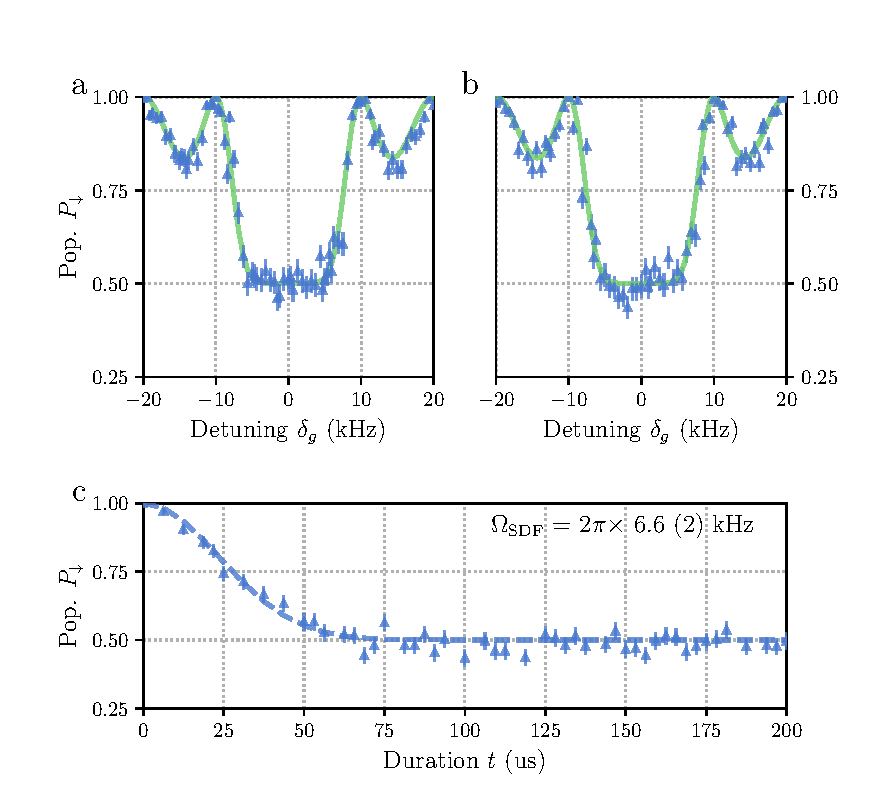
\includegraphics[width=\linewidth]{
            figures/pdf_figure/sdf.pdf
            }
        \end{center}
        \caption{
            SDF traces.
            }
        \label{fig:SDF}
    \end{figure}

    The MS interaction is widely used in ion trap experiments due to it being robust against varying intial motional states, and to the effects of heating during the pulse sequence. However, in our use case, the SDF is sensitive to various frequency and power miscalibrations and drifts of these between calibrations.  Here we describe briefly the work flow for calibrating and optimising the SDF behaviour.\\
    In honesty, there are not many moving parts in the SDF interaction, we must know the central qubit frequency, the motional mode frequency, the power in each tone, and the durations of the pulses. Complications come from the reality that we have a multi-level system, multiple motional modes, and that experimentally each parameter can only be controlled to a certain precision.\\
    We negate the effect of nearby motional modes by either selecting our
    interaction mode to be well seperated from the others either in frequency or geometrically, by
    operating the SDF near to resonance of the desired mode, or by using pulse
    shaping to ramp the power of the SDF and suppress the off-resonant
    excitation of these other modes. There are many tricks to either mitigate or
    exploit the effects of these other modes, and we will not go into detail
    here. \\
    The power balance of the SDF tones is complicated due to our use of AOMs.
    AOMs generate frequency shifts in the laser beam at the expense of small
    frequency-dependent angular shifts. We couple the beam after the AOM into a
    single mode fibre (see figure~\ref{fig:729}), and so the AOMs effectively introduce a
    frequency-dependent loss. To calibrate the power balance we look at a pick
    off of the bichromatic beam before the ion on a high bandwidth photodiode.
    We measure the beatnote contrast of the two tones and optimise the power
    balance to maximise this contrast.\\
    The far off-resonant levels of our ion lead to light-shifts of our qubit
    frequency. Practically to account for the light-shift we must calibrate this central frequency at the
    optical power we use in the interaction. We do this with the SDF interaction
    itself. When the qubit frequency is set incorrectly, the two tones will no
    longer have the same absolute detuning from their respective RSB or BSB.
    This manifests as a ``skewness'' of the SDF detuning trace, an example of
    such can be seen in figure~\ref{fig:SDF}. By varying the qubit frequency and
    inspecting these detuning scans, the desired SDF behaviour can be found. \\
    To verify the behaviour of our calibrated SDF with theory, we use both
    ``detuning'' and ``duration'' scans. The ``detuning'' scan is performed by
    varying the detuning, $\delta_g$, of the interaction, whilst the keeping the
    SDF duration, $t$, constant, and vice-versa for the ``duration'' scan. \\
    Figure~\ref{fig:SDF} shows the measured duration scan with a fit given by,
    \begin{equation}
        P_{\downarrow,\mathrm{th}} = \frac{1}{2} \left[ 1 + e^{-4\left( \bar{n} + \frac{1}{2} \right) |\alpha(t)|^2} \right],
    \end{equation}
    %from Burd thesis, equation 3.30.
    where we assume we begin in a thermal state with average Fock state $\bar{n}
    = 0.03$ which we found previously from thermometry measurements. Here the
    displacement, $|\alpha(t)| = \Omega_{\rm SDF} t/2$, where $\Omega_{\rm SDF}$ is the
    SDF amplitude. 
    These measurements were performed with a duration of XX~ms, total power of xx~mW, $\delta_{\rm LS}=2\pi\times XX$~kHz.
    We find $\Omega_{\rm SDF} = 2\pi\times 6.6(2)$~kHz, from the
    measured fit, which is in good agreement with the expected value of
    $\Omega_{\rm SDF} = \eta\Omega_{\rm CAR}$, where Lamb-Dicke parameter $\eta =
    0.05$XXX and $\Omega_{\rm CAR} = 2\pi \times 132$~kHz XXX measured from Rabi
    flopping at 15XXX mW.\\
    The detuning scan, shown in figure~\ref{fig:SDF}, is fitted by taking the
    displacement to be $|\alpha(t)| = \Omega_{\rm SDF} \sin(\delta t/2)/\delta$. Here
    we qualitatively see a good agreement between the measured data and the
    expected behaviour, with the main important features being the ``closure''
    at $\delta = 2\pi/t$ where the motional state returns to the initial state,
    and the central flat region around $P_{\downarrow, \mathrm{th}} =0.5$ where
    the two motional wave packets are non-overlapping.\\
    % find $\Omega_{SDF} = 2\pi\times 6.3(2)$~kHz, fitted with $\bar{n} = 0.03$.


\section{Two-Qubit Entangling Gates}
\label{sec:Two-Qubit Entangling Gates}
% Main points:
    % Intro/brief outline of goal of two-qubit gate. Truth table? Preparing in Bell state. This is tool kit for spin control of our system.
    % Discuss likely limitations being nearby hot motional modes, no pulse ramping
    % Current error vs what we expect we need for future experiments.
    % Here empasise that the SDF we discuss previously can be used to generate entanglement.
    % Showing phase coherence between operations is nice here.
% Prereqs:
    % SDFs
    % Single qubit gates
    % What available transitions we have
    % Motional mode spectra

    \begin{figure}
        \begin{center}
        \noindent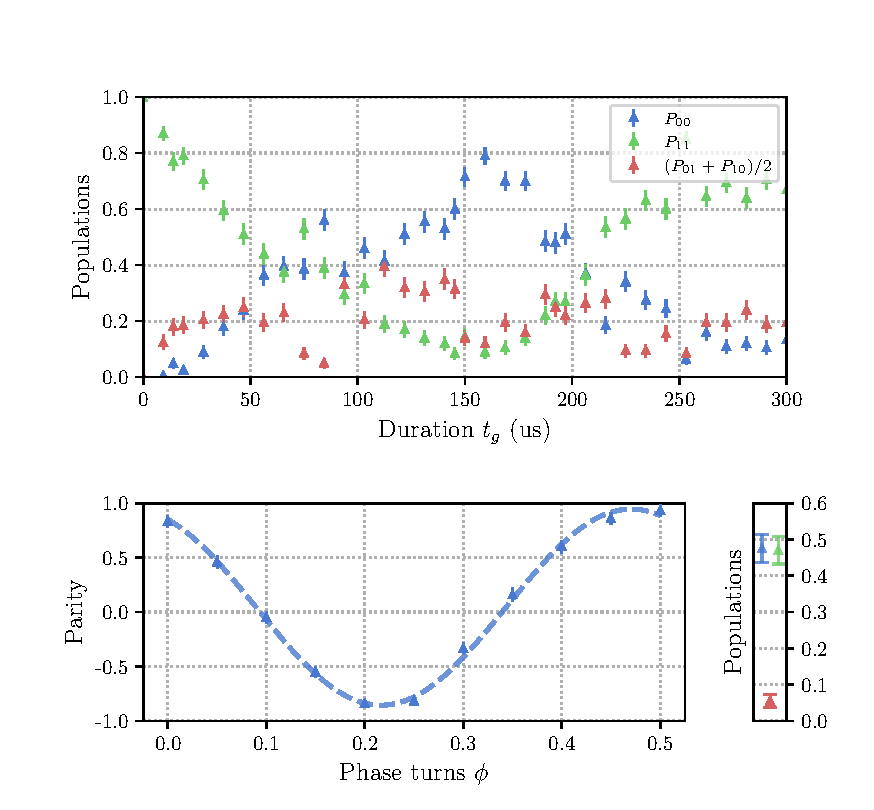
\includegraphics[width=\linewidth]{
            figures/pdf_figure/ms_gate.pdf
            }
        \end{center}
        \caption{
            MS Gate.
            }
        \label{fig:ms_gate}
    \end{figure}

    We perform two-qubit entangling gates using the Mølmer-Sørensen (MS)
    interaction~\cite{}. This interaction is the same described SDF from the
    previous section, but applied globally to two ions. The MS interaction
    relies on the spin dependent geometric phase accumulated during the motional
    displacement. To create a two-qubit entangled state, a differential
    geometric phase of $\pi/2$ must be accumulated between the two-qubit basis
    states. To ensure there is no residual motional entanglement, the final
    motional state must return to the initial state. In practise, using an SDF
    detuned by $\delta_g$, this is achieved by applying the MS interaction for a
    time $t = 2\pi/\delta_g$. The MS gate is a universal two-qubit gate, and
    along with only single qubit gates, constitutes a universal gate set for
    discrete quantum algorithms.\\  

    Here we quote the fidelity of experimentally demonstrated two-qubit gates on
    our system. The fidelity serves to quantify the ``closeness" or similarity of
    two density matrices.  For the use case of quantum information processing, what we
    care about is that the experimental unitary applied in the gate sequence closely resembles the unitary we desire theoretically. In general this
    means that we should measure the fidelity of the applied unitary in an input
    state agnostic way. Unfortunately this is often not practical as the input
    state space can be unwieldly, and the act of preparing the input state can
    also be error prone. As a compromise we can apply the test unitary to either
    one, or to a set of input states, and measure the fidelity of the output state
    with respect to the known target state. If the error mechansisms of the test
    unitary are well understood, arguments can be made that this measured
    fidelity for a set of input state is representative (or not representative)
    of the average fidelity over the input state space.\\
    Here for a two-qubit entangling gate, we target the creation of the Bell
    state $|\Phi^+\rangle = 1/\sqrt{2} \left( |00\rangle +
    e^{i\phi_0}|11\rangle \right)$, from an initial state of $|11\rangle$.
    The fidelity between our mixed state $\rho$, and the pure Bell state may be
    given by,
    \begin{equation}
        \mathcal{F} = \langle \Phi^+ | \rho | \Phi^+ \rangle = \frac{1}{2} \left( \rho_{00,00} + \rho_{11,11} \right) + \frac{1}{2}\left( e^{i\phi_0}\rho_{11,00}+e^{-i\phi_0}\rho_{00,11}\right),
        \label{eq:Fidelity}
    \end{equation}
    To extract the fidelity experimentally we follow the popular
    protocol~\cite{XXX}, where the first bracketted term of
    equation~\ref{eq:Fidelity} is measured by performing projective measurements
    of the two ions after the gate sequence to extract populations, and the second bracketted term,
    known as the coherence terms, are measured by applying a global analysis
    $\pi/2|_\phi$ pulse to the two ions and applying parity measurements. The
    contrast of the parity oscillations when varying the phase $\phi$ of the
    $\pi/2$ pulse yields the desired coherence term magnitude and phase. We require the creation of a Bell state for two qubit entangling, however do not care what basis this state is in, and so float the target Bell state phase and take only the magnitude of the fitted parity oscillations for calculating the final fidelity.\\

    The best two-qubit entangling gate fidelity currently achieved on our system is $\mathcal{F}=92(2)\%$. As shown in figure~\ref{fig:ms_gate}, the magnitude of the parity scan was measured to be 0.90(2), while the populations $\left( \rho_{00,00} + \rho_{11,11} \right) = 0.95(2)$. Each population point in these figures are found by taking the average of 200 shots of the gate sequence.\\

    These results serve as both a proof of principle for full spin control on
    our system, but also as a benchmark to which we can compare future system
    improvements.  For future work, we will require the use of this entangling
    gate either as Bell state preparation for input to analogue simulation
    experiments~\cite{}, or as a primitive gate for the spin component of hybrid
    algorithms~\cite{}.  In both these cases, especially any use that requires
    multiple concatenated entangling gates, we will likely require improved gate
    fidelities. It is suspected that we are currenlty limited by nearby hot
    motional modes, and the lack of pulse ramping in our gate sequence. We
    expect that with the addition of pulse shaping we will be able to suppress
    the effect of nearby off-resonant transitions, and by sideband cooling of
    nearby motional modes we will futher suppress contributions from unwanted
    spin-motion couplings.\\
